\section{Backgrounds}
\label{sec:bkg}
\subsection{vdM background}

The cluster rate equation is modified in the presence of background events.\\

N = \sigma \:L_{int} + N_{bg} \\

N: total number of signal and background events. \\

$N_{bg}$: Number of background events \\

$N_{bg}$ need to be subtracted during vdM scans for precise determination of $\sigma_{vis}$. These contributions to the measured cluster rate are either subtracted before the fit as measured from noncolliding, unpaired bunches or from periods during which the beams were kept at a large distance, or determined in the fit as a constant term added to the fit function as shown in Fig. 15.

\begin{figure}[H]
  \centering
  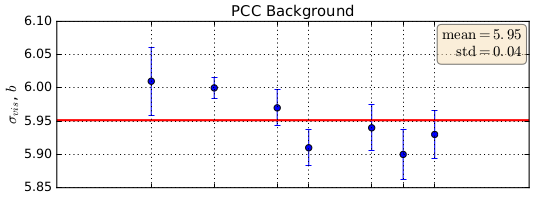
\includegraphics[width=0.7\columnwidth]{./PCC_bg.png}
  \caption{ \onehalfspacing Visible cross section $\sigma_{vis}$ with only background subtraction.}
  \label{fig:CMS}
\end{figure}


\subsection{High pileup physics run background}

During high pileup physics runs, background contribution to instantaneous luminosity based on the pixel cluster counting (PCC) method arises from a small out-of-time response (OOTR, or afterglow) that has two types.\\

Type I: fake hits in the bunch crossing after the colliding bunches (signal charge spillover).\\

Type II: Activated material in the detector due to the large radiation doses, exponentially decays for many bunch crossings.\\

Fig. 16 shows the afterglow noise induced by one colliding bunch. Since the distribution is normalized to 1 at the first bin it means the first bin is the colliding bunch. The values at bins greater than 1 are the cluster counts observed for bunches after the colliding bunch divided by the cluster counts observed by the colliding bunch. There are three parts to this distribution: \\

(i) bin 1 is the colliding bunch \\

(ii) bin 2 (empty bunch) is the bunch after colliding bunch, noise observed is due to electronics signal on same pixels from colliding bunch. This is Type I afterglow effect. \\

(iii) bins greater than 2 are all empty bunches. Noise observed is due to "albedo" which is material activated by the radiation of the collisions, it decays exponentially with time just like radioactive material. It produces secondary particles which create hits late in time. This is called Type II afterglow effect. \\

\begin{figure}[H]
  \centering
  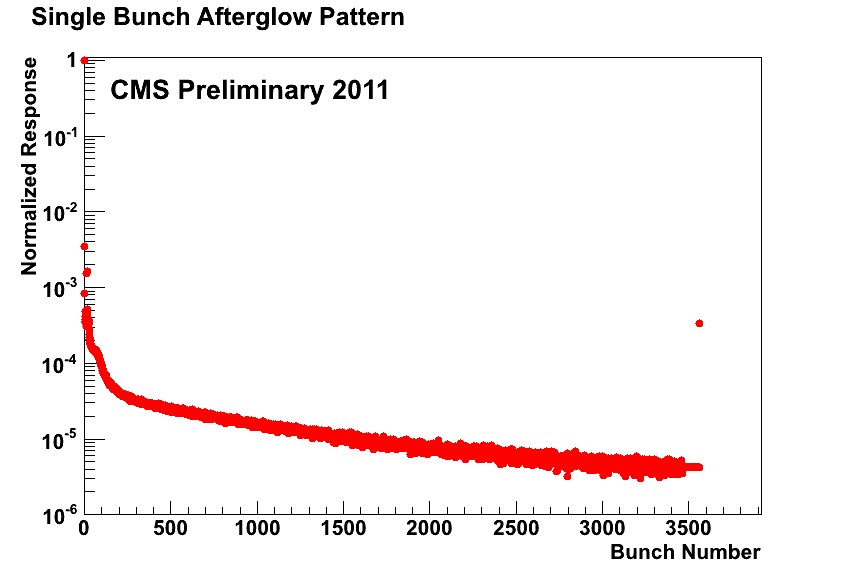
\includegraphics[width=0.6\columnwidth]{./SingleBunchAfterglow.png}
  \caption{Afterglow effect produced by a single colliding bunch.}
  \label{fig:LHC}
\end{figure}

 Afterglow effects for various bunches in a beam is shown in Fig. 17 where the intial rising curve correspond to Type I and decay curve correspond to Type II afterglow effect. It was studied in data taken using random triggers (triggers that fire randomly in bunch crossings spread over the whole LHC orbit except for the abort gap), considering the pixel cluster counts in bunch crossings after bunch trains. The resulting correction depends on the LHC filling scheme and for a typical 2011 fill with 1380 bunches corresponds to a subtraction of close to 2.8$\%$ of the integrated luminosity per lumi section. The afterglow corrections for PCC during 2017 run are in the range 2-5 $\%$ for the Type I corrections and 2-3 $\%$ averaged over all active bunches for the Type II corrections \cite{Sirunyan:2759951}.



\begin{figure}[H]
  \centering
  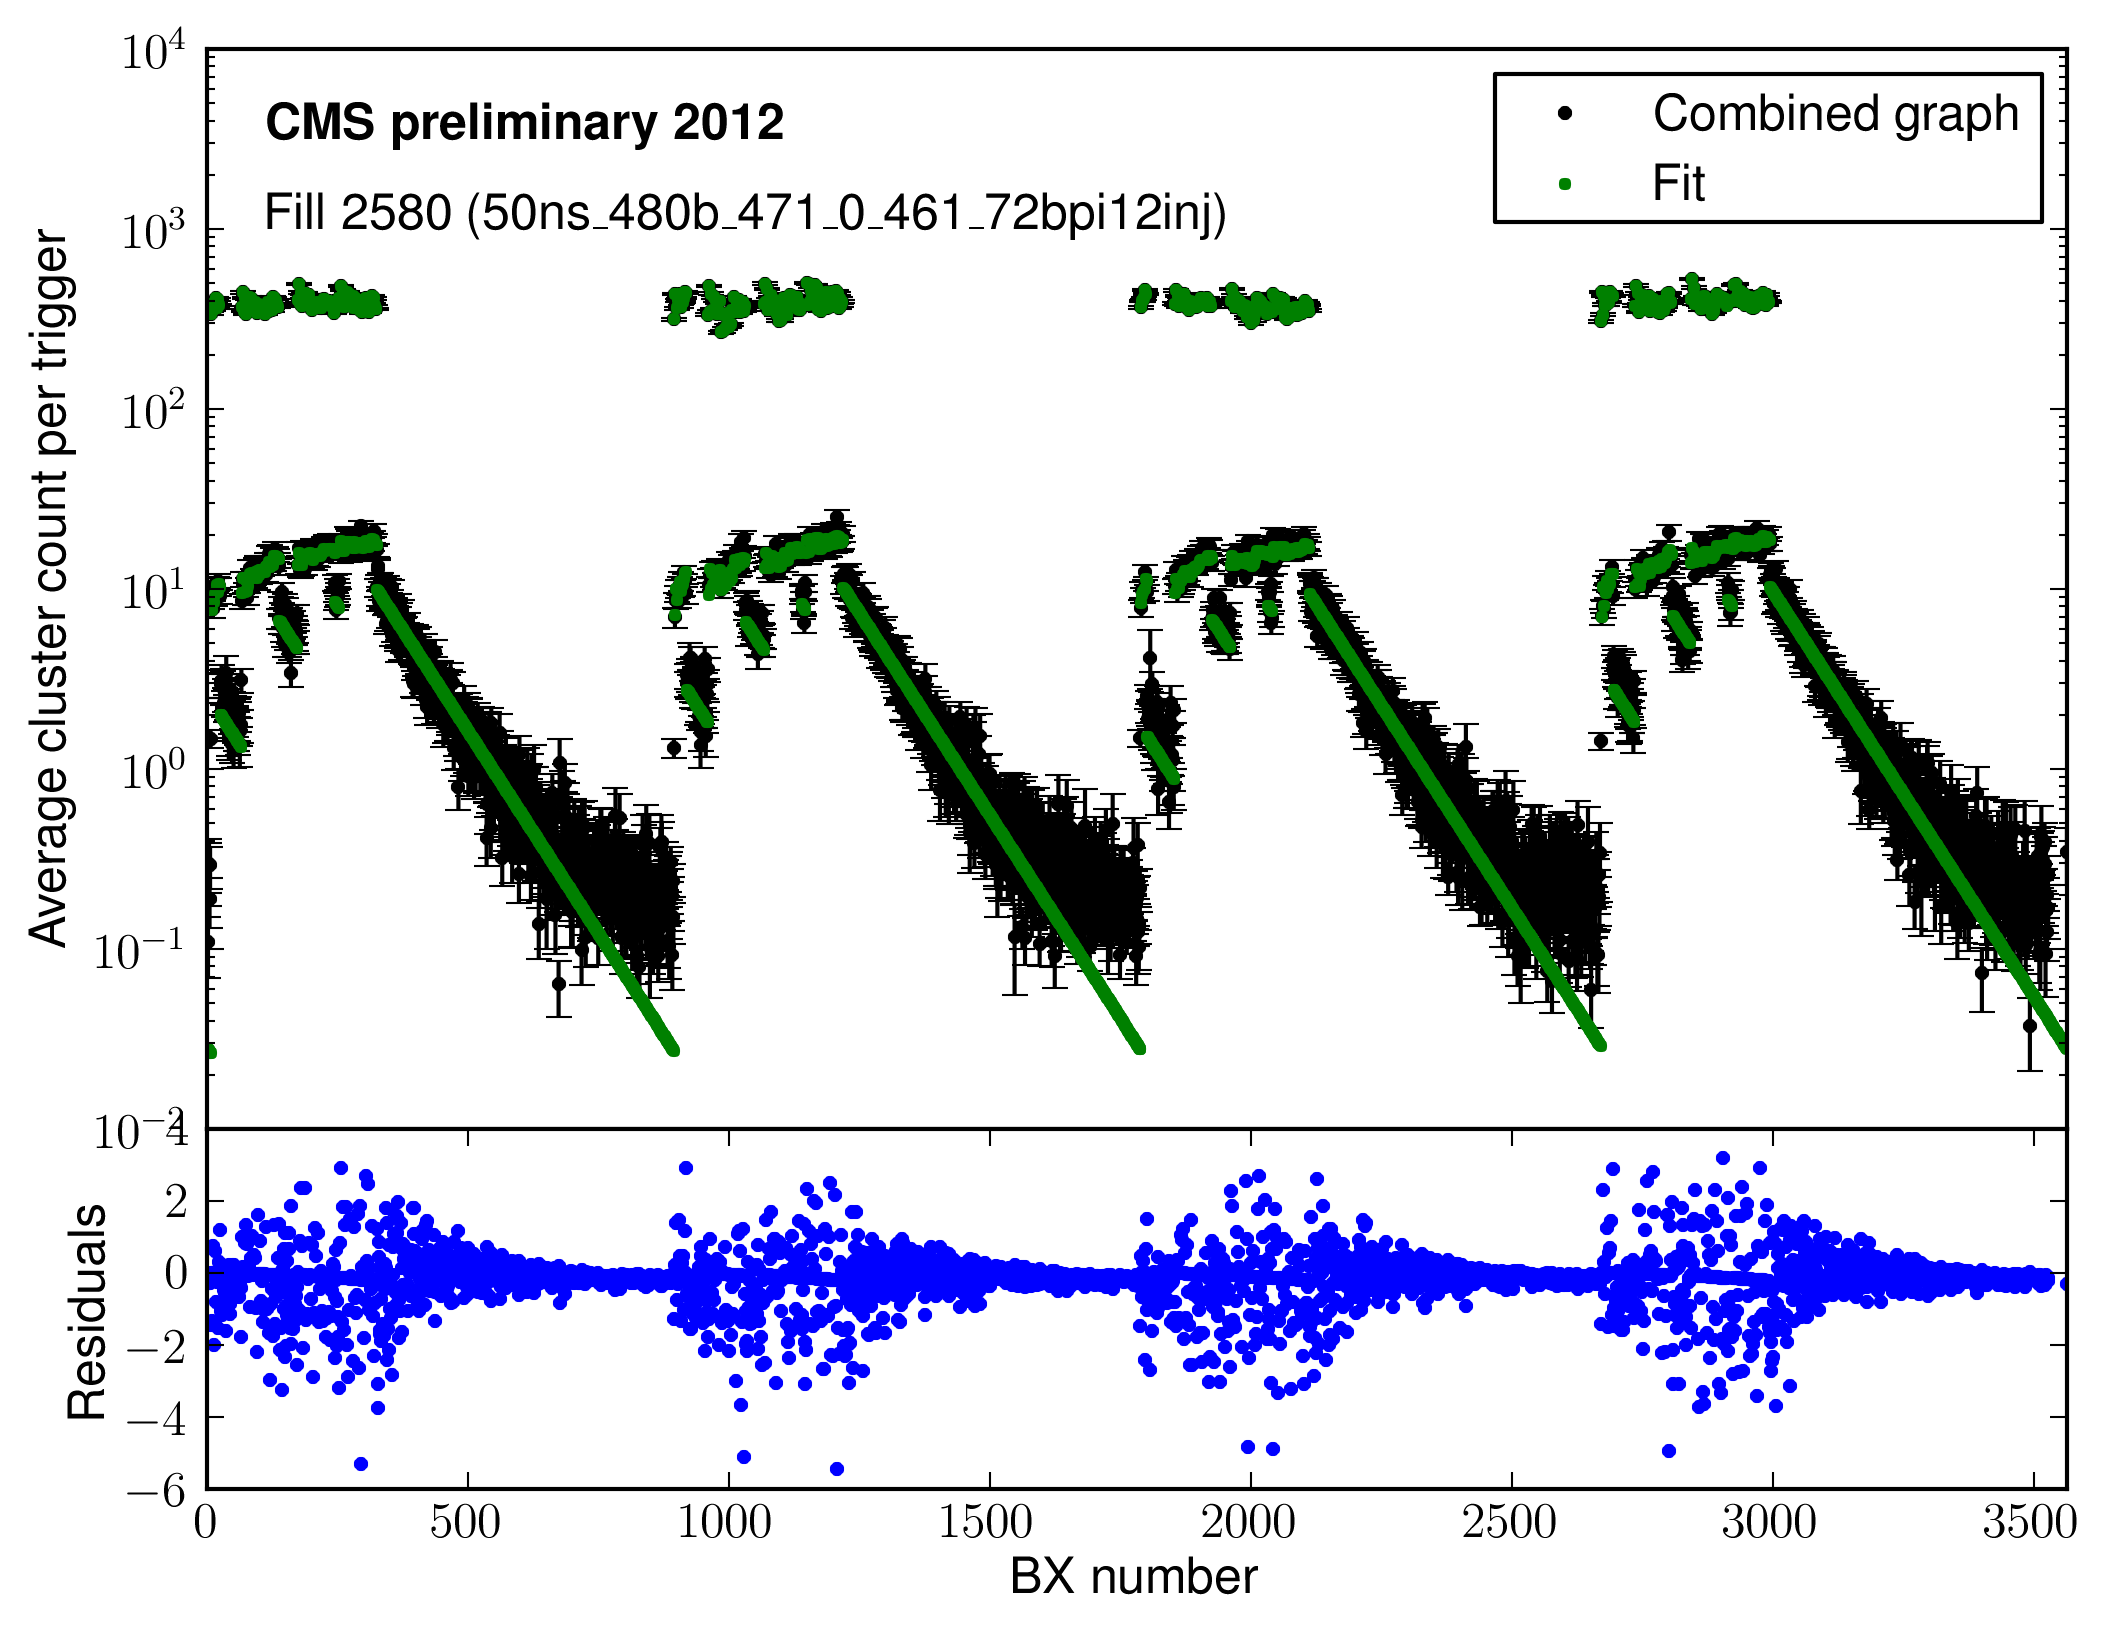
\includegraphics[width=0.5\columnwidth]{./afterglow.png}
  \caption{Results of the pixel afterglow fit. Type I afterglow effect results from fake electronic pulse response after actual bunch crossing and Type II results from activation of detector material shown as exponentially decaying. }
  \label{fig:LHC}
\end{figure}




\clearpage\newpage
